\begin{sidewaysfigure}[htbp]
\centering 
  \subfloat%[Jenike shear cell tester.]
  {
	  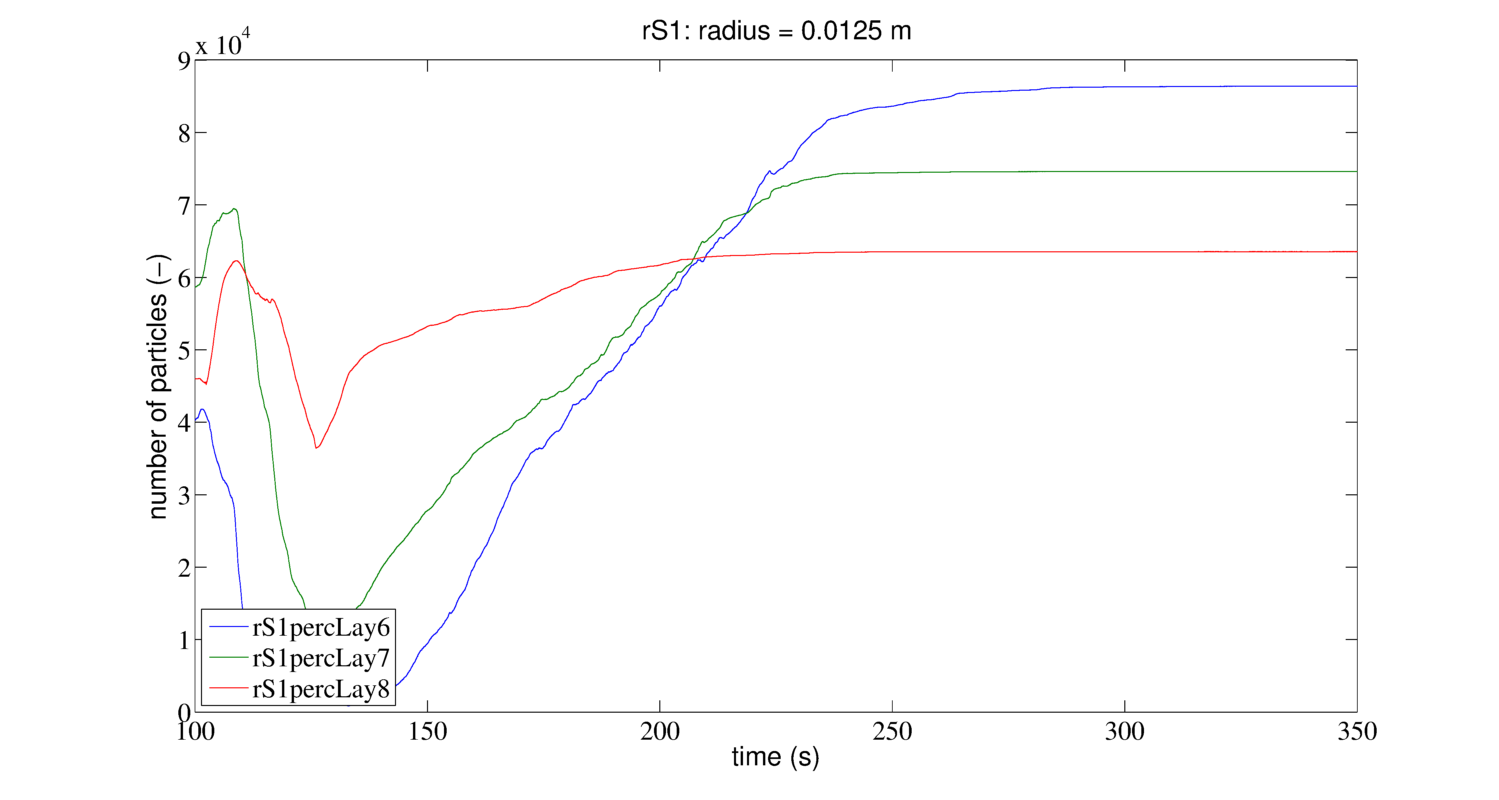
\includegraphics[width=.48\columnwidth]{images/114rS120151111151255}
	  \label{fig:114rS120151111151255}
  }
  \quad
    \subfloat
    %[Simplified Jenike shear cell tester.]
    {
	  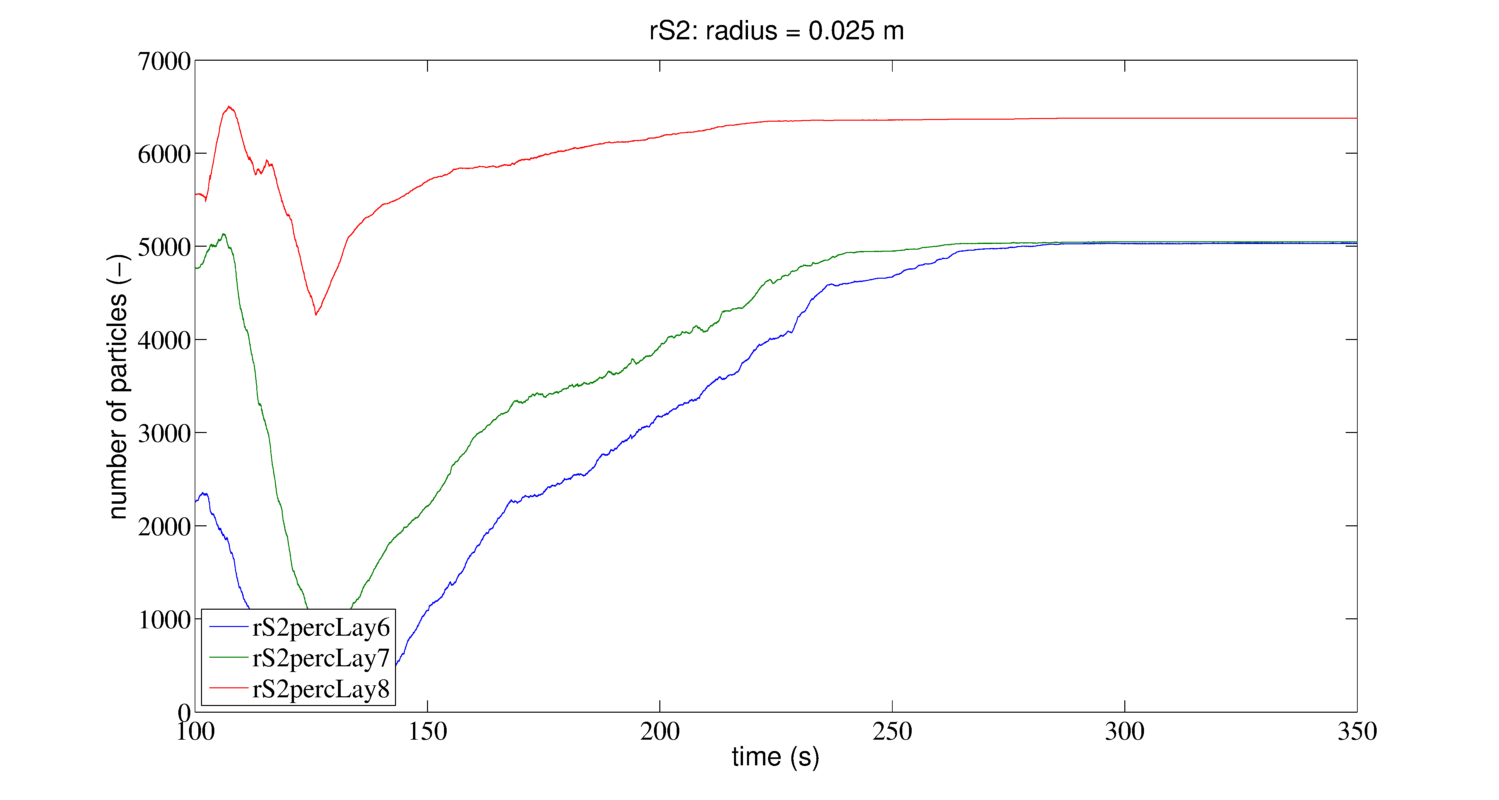
\includegraphics[width=.48\columnwidth]{images/116rS220151111151255}
	  \label{fig:116rS220151111151255}
  }
  \\
  \subfloat%[Jenike shear cell tester layout.]
  {
	  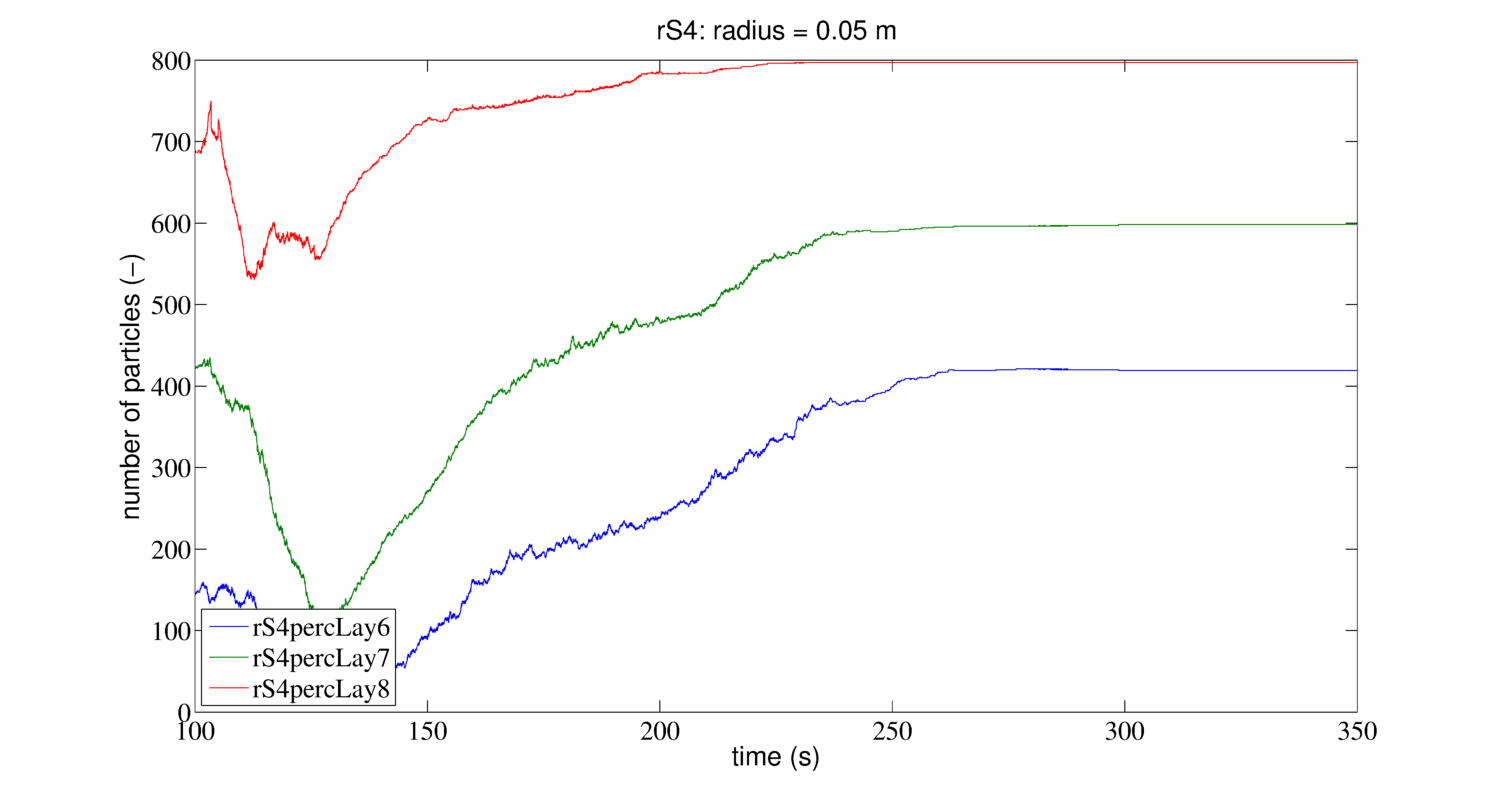
\includegraphics[width=.48\columnwidth]{images/118rS420151111151255}
	  \label{fig:118rS420151111151255}
  }
  \quad
    \subfloat%[Jenike shear cell tester diagram.]
    {
	  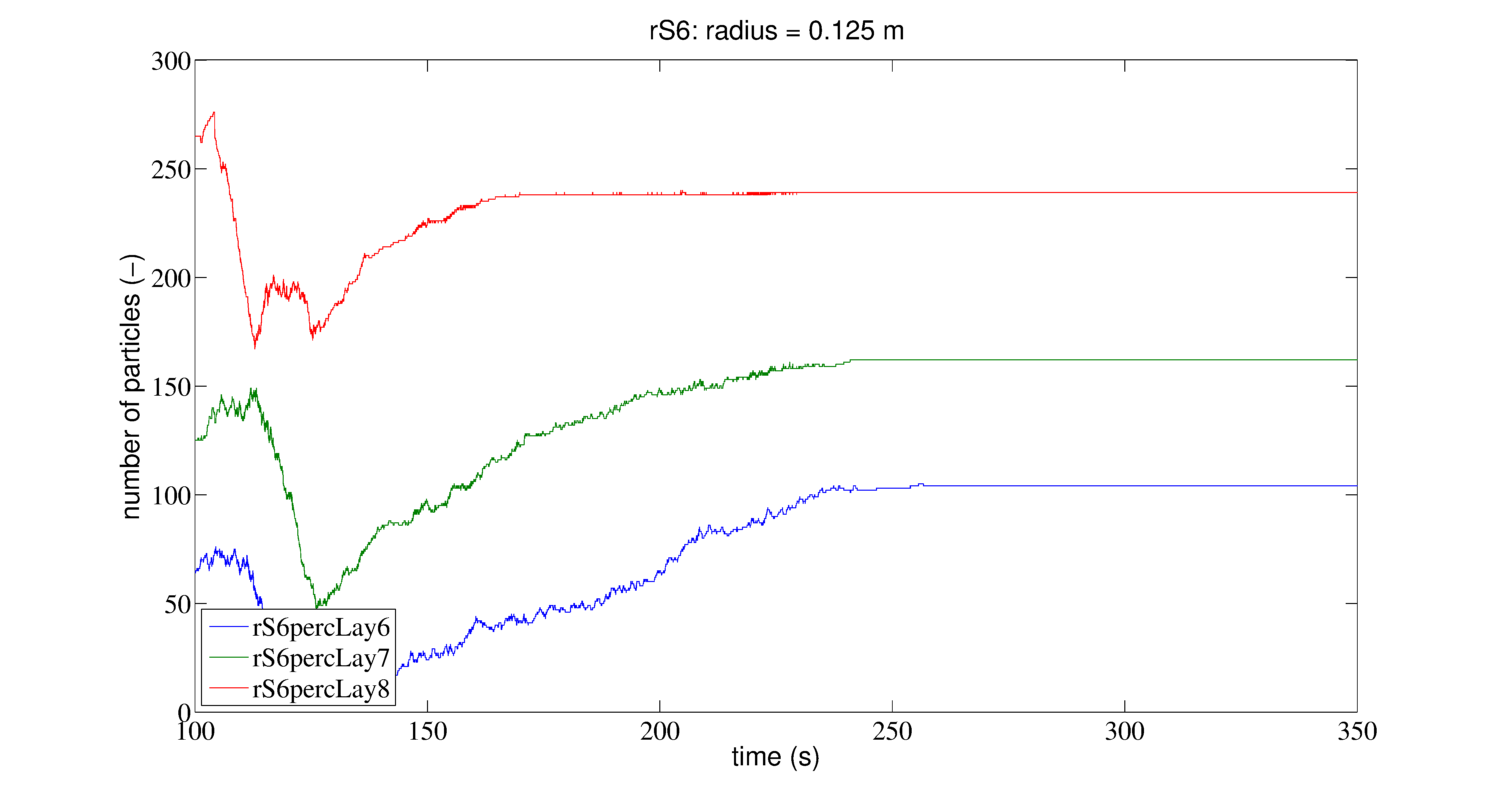
\includegraphics[width=.48\columnwidth]{images/120rS620151111151255}
	  \label{fig:120rS620151111151255}  }
  \\
  \caption{Particle size distribution during the simulation, number of
  particles. Once steady state is reached, large particles are more likely in the
  inferior layers, small particles in the superior ones.}
  \label{fig:223sinterplots2}
\end{sidewaysfigure}